\section{Implementation}
\label{section:implementation}

%\begin{enumerate}
%	\item Überlick über eure Implementierung
%	\item Modell der Softwarearchitektur
%\end{enumerate}

We first implemented a script to fuzz a CoAP server. The workflow of that script is shown in \Autoref{figure:fuzz_flow_chart}. As we described in \Autoref{section:background}, we use \scapy and its CoAP community contribution\footnote{\url{https://github.com/secdev/scapy/blob/master/scapy/contrib/coap.py}} to create crafted CoAP packets. We test the availability of the IoT device after each crafted packet by sending a CoAP request to the URI ``/.well-known/core`` as we reported in \Autoref{section:approach}. We log the timestamp, the fuzzed request, its response and the result of the ``well-known-core`` check for each crafted packet.

\begin{figure*}
	\centering
	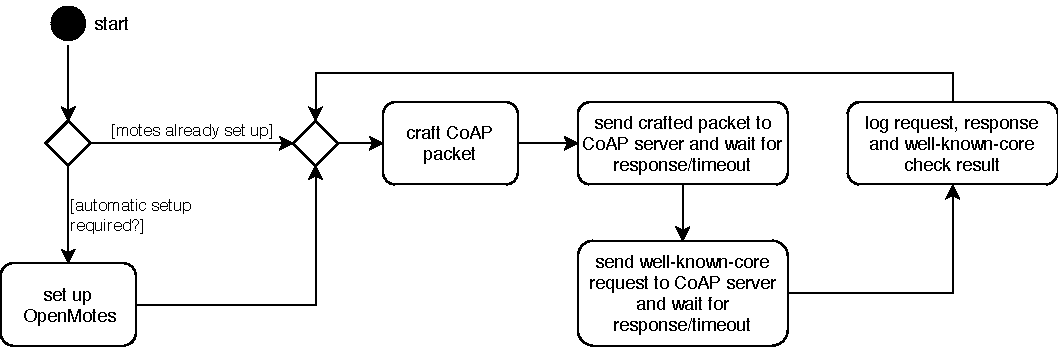
\includegraphics[width=\textwidth]{images/fuzzing_flow_chart}
	\caption{Flow chart of the fuzzing script}
	\label{figure:fuzz_flow_chart}
\end{figure*}

The CoAP implementation of Contiki-NG actually not only implements the CoAP RFC but it also implements extension RFCs, like the Block-Wise Transfers RFC\footnote{\url{https://tools.ietf.org/html/rfc7959}}. This means that the first response to the ``well-known-core``request contains only the first 64 bytes of the response and an option that more packets follow. But the CoAP community contribution of \scapy does not implement any extension RFCs of CoAP and therefore it does not support the Block-Wise Transfer RFC. This results in us only being able to test the first 64 bytes of the response to the ``well-known-core`` request unless we implement the Block-Wise Transfers RFC ourselves. But for our purposes it's enough to simply compare the first 64 bytes of the response.

We also implemented a second script that is able to replay a request that we logged in our first script and it then displays the response and the result of the ``well-known-core`` check. We created this script to test the reproducibility of a request that resulted in a device malfunction. We also added a simple error to the CoAP implementation of Contiki-NG to test if we were able to find such an error. This error caused the hardware watchdog to restart the CoAP server. We were indeed able to find this error.

For convenience we also created bash scripts to automatize the setup of the OpenMotes with the border router and the CoAP server. This enables us to start fuzzing by simply connecting the two OpenMotes to our computer and then just running a single command, which is our python script.
